\documentclass{beamer}

\usepackage{verbatim}
\usepackage{fancyvrb}
\usepackage{amsmath}
\usepackage{mathtools}
\usepackage{booktabs}
\usepackage{amssymb}
\usepackage{graphicx}
\usepackage{calc}
\usepackage{color}
\usepackage{multicol}
\usepackage{wrapfig}
\usepackage{natbib}
\usepackage[ruled,vlined]{algorithm2e}
\usepackage{animate}
\usepackage{mathtools}
\usepackage{listings}
\usepackage{xfrac}

% two col: two columns
\newenvironment{twocol}[4]{
\begin{columns}[c]
\column{#1\textwidth}
#3
\column{#2\textwidth}
#4
\end{columns}
}

\makeatletter
\setbeamertemplate{theorem begin}
{%
\begin{\inserttheoremblockenv}
  {}{\usebeamerfont*{block title}\usebeamercolor[fg]{block title}%
  \inserttheoremname
  %\inserttheoremnumber
  \ifx \inserttheoremaddition \empty \else\ (\inserttheoremaddition)\fi
  \inserttheorempunctuation}
  \normalfont
  }
  \setbeamertemplate{theorem end}{\end{\inserttheoremblockenv}}
\makeatother

\newcommand{\E}{\mathrm{E}}
\newcommand{\Var}{\mathrm{Var}}
\newcommand{\Cov}{\mathrm{Cov}}
\newcommand{\s}{\mathrm{s}}
\newcommand{\Corr}{\mathrm{Corr}}
\newcommand{\rank}{\mathrm{rank}}
\newcommand{\nullspace}{\mathrm{null}}
\newcommand{\myspan}{\mathrm{span}}
\DeclareMathOperator*{\argmax}{arg\,max}
\DeclareMathOperator*{\argmin}{arg\,min}
\DeclareMathOperator*{\softmax}{softmax}

\definecolor{darkgreen}{rgb}{0,0.5,0}

\newtheorem{prop}[theorem]{Proposition}
\newtheorem{exe}{Exercise}
\newtheorem{remark}{Remark}
\newtheorem{myproof}{Proof}

\definecolor{darkgreen}{rgb}{0,0.5,0}

\title{Inferences in Regression Analysis}
\author{Zhenisbek Assylbekov}
\institute{Department of Mathematics}
\date{Regression Analysis}

\AtBeginSection[]
{
  \begin{frame}<beamer>
    \tableofcontents[currentsection]
  \end{frame}
}

\begin{document}

\begin{frame}
  \titlepage
\end{frame}

\begin{frame}{Normal Errors Regression}
    Throughout this chapter we assume
    \begin{align*}
    &Y_i=\beta_0+\beta_1 x_i+\epsilon_i,\\
    &\epsilon_1,\ldots,\epsilon_n\stackrel{\rm iid}{\sim}\mathcal{N}(0,\sigma^2).
    \end{align*}
    \pause{This is equivalent to
    $$
    Y_i\,{\stackrel{\text{ind}}{\sim}}\,\mathcal{N}(\beta_0+\beta_1 x_i,\sigma^2)
    $$}
\end{frame}

\section{Inferences on $\beta_1$ and $\beta_0$}

\begin{frame}{Unbiasedness of $b_1$}
\begin{prop}
$b_1$ is an unbiased estimator of $\beta_1$.
\end{prop}
\pause\begin{proof}
Recall that $b_1=\frac{\sum(x_i-\bar{x})(Y_i-\bar{Y})}{\sum(x_i-\bar{x})^2}\pause{\stackrel{\text{?}}{=}\frac{\sum(x_i-\bar{x})Y_i}{\sum(x_i-\bar{x})^2}}$.

\pause Expected value of the numerator is
\begin{align}
&\E\left[\sum(x_i-\bar{x})Y_i\right]=\sum(x_i-\bar{x})\E[Y_i]=\sum(x_i-\bar{x})(\beta_0+\beta_1 x_i)\notag\\
&=\beta_0\sum x_i-n\bar{x}\beta_0+\beta_1\sum x_i^2-n\bar{x}^2\beta_1=\beta_1\left(\sum x_i^2-n\bar{x}^2\right)\label{eq:numerator}\notag
\end{align}
\pause The denominator is
$$
\sum(x_i-\bar{x})^2=\sum x_i^2-2\sum x_i\cdot\bar{x}+\sum\bar{x}^2=\sum x_i^2-n\bar{x}^2
$$
\pause Hence, $\E[b_1]=\beta_1$.
\end{proof}
\end{frame}

\begin{frame}{Variance of $b_1$}
\begin{prop}
$\Var[b_1]=\frac{\sigma^2}{\sum_{i=1}^n(x_i-\bar{x})^2}.$
\end{prop}
\pause\begin{proof}
\begin{align*}
\Var[b_1]&=\Var\left[\frac{\sum_i (x_i-\bar{x})Y_i}{\sum_i (x_i-\bar{x})^2}\right]\onslide<3->{=\frac{\sum_i(x_i-\bar{x})^2\Var[Y_i]}{\left[\sum_i(x_i-\bar{x})^2\right]^2}\\}
\onslide<4->{&=\frac{\sigma^2\sum_i(x_i-\bar{x})}{\left[\sum_i(x_i-\bar{x})^2\right]^2}}\onslide<5->{=\frac{\sigma^2}{\sum_{i=1}^n(x_i-\bar{x})^2}.}
\end{align*}
\end{proof}
\onslide<6->{\begin{remark}
\begin{itemize}
    \item<6-> $\sum_i{(x_i-\bar{x})^2}\uparrow$\quad $\Rightarrow$\quad $\Var[b_1]\downarrow$
    \item<7-> $n\uparrow\quad\Rightarrow\quad\Var[b_1]\downarrow$
\end{itemize}
\end{remark}}
\end{frame}

\begin{frame}{Distribution of $b_1$}
Rewrite $b_1$ as
$$
b_1=\frac{\sum_i(x_i-\bar{x})Y_i}{\sum_i(x_i-\bar{x})^2}=\sum_{i=1}^n\left[\frac{(x_i-\bar{x})}{\sum_{j=1}^n(x_j-\bar{x})^2}\right]Y_i
$$%
\onslide<2->{Thus, $b_1$ is a linear combination of $n$ independent normal random variables $Y_1,\ldots,Y_n$.} \onslide<3->{Therefore}
$$
\onslide<3->{b_1\sim}\onslide<4->{\mathcal{N}\left(\beta_1,\frac{\sigma^2}{\sum_{i=1}^n(x_i-\bar{x})^2}\right),}
$$%
\onslide<5->{and
$$
\frac{b_1-\beta_1}{\sqrt{\Var[b_1]}}\sim\mathcal{N}(0,1).
$$}%
\onslide<6->{We never know $\sigma^2$, we estimate it by MSE $=\frac{1}{n-2}\sum_i (Y_i-\hat{Y}_i)^2$.}
\end{frame}

\begin{frame}{Distribution of $\frac{b_1-\beta_1}{\s[b_1]}$}
Denote $
\s[b_1]=\sqrt{\frac{\text{MSE}}{\sum_{i=1}^n(x_i-\bar{x})^2}}$.
\pause\begin{theorem}
$\frac{b_1-\beta_1}{\s[b_1]}\sim t_{n-2}.$
\end{theorem}
\begin{proof}
\begin{align*}
\frac{b_1-\beta_1}{\s[b_1]}&=\overbrace{\frac{b_1-\beta_1}{\sqrt{\Var[b_1]}}}^{Z}\cdot\frac{\sqrt{\Var[b_1]}}{\s[b_1]} =Z\cdot\sqrt{\frac{\sigma^2}{\frac{1}{n-2}\sum_i{e_i^2}}}\\
&=\frac{Z}{\sqrt{\frac{\sfrac{\sum_i e_i^2}{\sigma^2}}{n-2}}}=\frac{Z}{\sqrt{\frac{\chi^2_{n-2}}{n-2}}}\sim t_{n-2},
\end{align*}
where we used the fact that $\frac{\sum_i e_i^2}{\sigma^2}\sim\chi^2_{n-2}$ (Ch 5).
\end{proof}
\end{frame}

\begin{frame}{Confidence interval for $\beta_1$ and testing $\rm{H}_0:\beta_1=\beta_{10}$}
A $(1-\alpha)\cdot100\%$ CI for $\beta_1$ has endpoints
$$
b_1\pm t_{n-2,1-\alpha/2}\cdot\s[b_1].
$$

\pause Under $\rm{H}_0:\beta_1={\beta_{1,0}}$,
$$
T=\frac{b_1-\beta_{1,0}}{\s[b_1]}\sim t_{n-2}.
$$
\pause P-values are computed as usually.\\~\\

\pause In simple linear regression
$$
Y_i=\beta_0+\beta_1 x_i+\epsilon_i
$$
of particular interest is $\rm{H}_0:\beta_1=0$, that $Y_i$ and \textit{does not depend on} $x_i$. 
\end{frame}

\begin{frame}{Expectation, Variance, and Distribution of $b_0$}
\begin{exe}
Show that
\begin{itemize}
    \item $\E[b_0]=\beta_0$
    \item<2->$\Var[b_0]=\left[\frac1n+\frac{\bar{x}^2}{\sum_i(x_i-\bar{x})^2}\right]\sigma^2$
    \item<3->$b_0\sim\mathcal{N}\left(\beta_0,\left[\frac1n+\frac{\bar{x}^2}{\sum_i(x_i-\bar{x})^2}\right]\sigma^2\right)$
    \item<4->$\frac{b_0-\beta_0}{\s[b_0]}\sim t_{n-2}$, where $\s[b_0]$ is obtained from $\sqrt{\Var[b_0]}$ when replacing $\sigma^2$ by MSE
\end{itemize}
\end{exe}%
\onslide<5->{CI and Hypothesis Test for $\beta_0$ are as usual.}
\end{frame}

\begin{frame}{Table of regression coefficients}
Regression output typically produces a table like:

\vspace{10pt}
\begin{small}
\begin{tabular}{c c c c c}
Parameter & Estimate & Standard error & $t^\ast$ & p-value\\
\hline
Intercept $\beta_0$ & $b_0$ & $\s[b_0]$ & $t^\ast_0=\frac{b_0}{\s[b_0]}$ & $\Pr(|T|>|t_0^\ast|)$\\
Slope $\beta_1$ & $b_1$ & $\s[b_1]$ & $t_1^\ast=\frac{b_1}{\s[b_1]}$ & $\Pr(|T|>|t_1^\ast|)$\\
\hline
\end{tabular}
\end{small}

\vspace{10pt}
\pause where $T\sim t_{n-p}$ and $p$ is the number of parameters used to estimate the mean, here $p=2$: $\beta_0$ and $\beta_1$. Later $p$ will be the number of predictors in the model plus one.

\vspace{10pt}
\pause The two p-values in the table test $\rm{H}_0:\beta_0=0$ and $\rm{H}_1:\beta_1=0$ respectively. The test for zero intercept is usually not of interest.
\end{frame}

\begin{frame}[fragile]{Regression Output in \texttt{R}: Poverty vs HS grad rate}

{\color{blue} \url{https://raw.githubusercontent.com/zh3nis/MATH440/main/chp01/poverty.R}}
\begin{small}
\begin{verbatim}
Coefficients:
            Estimate Std. Error t value Pr(>|t|)    
(Intercept) 64.78097    6.80260   9.523 9.94e-13 ***
Graduates   -0.62122    0.07902  -7.862 3.11e-10 ***
---
Signif. codes:  0 ‘***’ 0.001 ‘**’ 0.01 ‘*’ 0.05 ‘.’ 0.1 ‘ ’ 1

Residual standard error: 2.082 on 49 degrees of freedom
\end{verbatim}
\end{small}
\pause We reject $\rm{H}_0:\beta_1=0$ at any reasonable significance level. There is a significant linear association between HS graduation and poverty rates.
\end{frame}

\section{Inferences on $\E[Y]$ and $\hat{Y}$}

\begin{frame}{Inference on $\E[Y]=\beta_0+\beta_1 x$}
Let $x$ be any value of the \textit{predictor}; we want to estimate the mean of all responses in the \textit{population} that correspond to $x$. This is given by
$$
\E[Y]=\beta_0+\beta_1 x.
$$
Our estimator of $\E[Y]$ is
\begin{align*}
\hat{Y}&=b_0+b_1 x\\
&=\sum_{i=1}^n\left[\frac1n-\frac{\bar{x}(x_i-\bar{x})}{\sum_{j=1}^n(x_j-\bar{x})^2}+\frac{(x_i-\bar{x})x}{\sum_{j=1}^n(x_j-\bar{x})^2}\right]Y_i\\
&=\sum_{i=1}^n\left[\frac1n+\frac{(x-\bar{x})(x_i-\bar{x})}{\sum_{j=1}^n(x_j-\bar{x})^2}\right]Y_i
\end{align*}
\end{frame}

\begin{frame}{Distribution of $\hat{Y}$}
\textit{Again} we have a linear combination of independent normals as our estimator. This leads, after some math, to
\begin{equation}
b_0+b_1 x\sim \mathcal{N}\left(\beta_0+\beta_1 x,\sigma^2\left[\frac1n+\frac{(x-\bar{x})^2}{\sum_{i=1}^n(x_i-\bar{x})^2}\right]\right).\label{eq:reg_dist}
\end{equation}

\pause As before, this leads to a $(1-\alpha)\cdot100\%$ CI for $\beta_0+\beta_1 x$
$$
b_0+b_1 x\pm t_{n-2,1-\alpha/2}\cdot\s[b_0+b_1 x],
$$
\pause where $\s[b_0+b_1 x]=\sqrt{\text{MSE}\cdot\left[\frac1n+\frac{(x-\bar{x})^2}{\sum_{i=1}^n(x_i-\bar{x})^2}\right]}.$\\~\\

\pause For what value of $x$ is the CI narrowest? \pause For $x=\bar{x}$.

\begin{exe}
Prove \eqref{eq:reg_dist}. \pause Solution is on pp. 53--54 of the textbook.
\end{exe}
\end{frame}

\begin{frame}{Prediction intervals}
\begin{itemize}
\item We discussed constructing a CI for the unknown $\E[Y]$ at $x$.
\item<2-> What if we want to find an interval that the actual \textit{value} $Y$ is in (versus only its mean) with fixed probability?
\item<3-> If we knew $\beta_0$, $\beta_1$, and $\sigma^2$ this would be easy, because
$$
Y=\beta_0+\beta_1 x+\epsilon\sim\mathcal{N}(\beta_0+\beta_1 x,\sigma^2),
$$
and a $(1-\alpha)\cdot100\%$ CI for $\E[Y]$ would be
$$
\beta_0+\beta_1 x\pm z_{1-\alpha/2}\cdot\sigma.
$$
\item<4-> Unfortunately, we don't know $\beta_0$, $\beta_1$, and $\sigma$, but we can estimate all three of these.
\end{itemize}
\end{frame}

\begin{frame}{Variability of $b_0+b_1 x + \epsilon$}
An interval that contains $Y$ with $(1-\alpha)$ probability needs to account for
\begin{itemize}
\pause\item the variability of the estimators $b_0$ and $b_1$
\pause\item the natural variability of response $Y$ built into the model: $\epsilon\sim\mathcal{N}(0,\sigma^2)$.
\pause We have
\begin{align*}
\Var[b_0+b_1 x + \epsilon]&=\Var[b_0+b_1 x]+\Var[\epsilon]\\
 &=\sigma^2\left[\frac1n+\frac{(x-\bar{x})^2}{\sum_{i=1}^n(x_i-\bar{x})^2}\right]+\sigma^2\\
 &=\sigma^2\left[\frac1n+\frac{(x-\bar{x})^2}{\sum_{i=1}^n(x_i-\bar{x})^2}+1\right]
\end{align*}
\end{itemize}
\end{frame}

\begin{frame}{Prediction interval}
Estimating $\sigma^2$ by MSE we obtain that a $(1-\alpha)\cdot100\%$ \textbf{prediction interval} (PI) for $Y$ is
$$
b_0+b_1 x\pm t_{n-2,1-\alpha/2}\sqrt{{\text{ MSE}}\left[\frac1n+\frac{(x-\bar{x})^2}{\sum_{i=1}^n(x_i-\bar{x})^2}+1\right]}.
$$
\begin{remark} As $n\to\infty$, we have $b_0\stackrel{\rm P}{\to}\beta_0$, $b_1\stackrel{\rm P}{\to}\beta_1$, $t_{n-2,1-\alpha/2}\to z_{1-\alpha/2}$, and ${\rm MSE}\stackrel{\mathrm{P}}{\to}\sigma^2$.\\~\\

I.e., as the sample size grows, the PI converges to
$$
\beta_0+\beta_1 x\pm z_{1-\alpha/2}\cdot\sigma.
$$
\end{remark}
\end{frame}

\begin{frame}{Example: Poverty vs HS Graduation data}
\begin{itemize}
\item Find a 95\% CI for the mean poverty rate $\E[Y]$ in a state with HS graduation rate $x=80$.
\item Find a 95\% PI for the poverty rate $Y$ in a state with HS graduation rate $x=80$.
\item \texttt{R} code follows\ldots
\end{itemize}
\end{frame}

\begin{frame}[fragile]
\frametitle{\texttt{R} code}
{\color{blue}\url{https://raw.githubusercontent.com/zh3nis/MATH440/main/chp02/pov_predict.R}}
\begin{footnotesize}
\begin{verbatim}
> poverty = read.table("path/to/poverty.txt", h = T, sep = "\t")

> my_model = lm(Poverty ~ Graduates, data=poverty)

> new_x = data.frame(Graduates=80)

> predict.lm(my_model, new_x, interval="confidence", level=0.95)
       fit     lwr      upr
1 15.08363 13.9636 16.20365

> predict.lm(my_model, new_x, interval="prediction", level=0.95)
       fit     lwr      upr
1 15.08363 10.7527 19.41455
\end{verbatim}
\end{footnotesize}

\pause A 95\% CI for $\E[Y]$ given $x=80$ is $[13.96, 16.20]$.\\
\pause A 95\% PI for $Y$ given $x=80$ is $[10.75, 19.41]$.
\end{frame}


\begin{frame}{Confidence Band for Regression Line}
\begin{columns}
\begin{column}{0.45\textwidth}
\textbf{Working-Hotelling} confidence band:
$$
\hat{Y}\pm W\cdot\s[\hat{Y}],
$$
where $W^2=2\cdot F_{1-\alpha; 2, n-2}$. \pause Gives region that \textit{entire} regression line lies in with certain confidence.
\end{column}%
\begin{column}{.55\textwidth}
\pause \begin{figure}
    \centering
    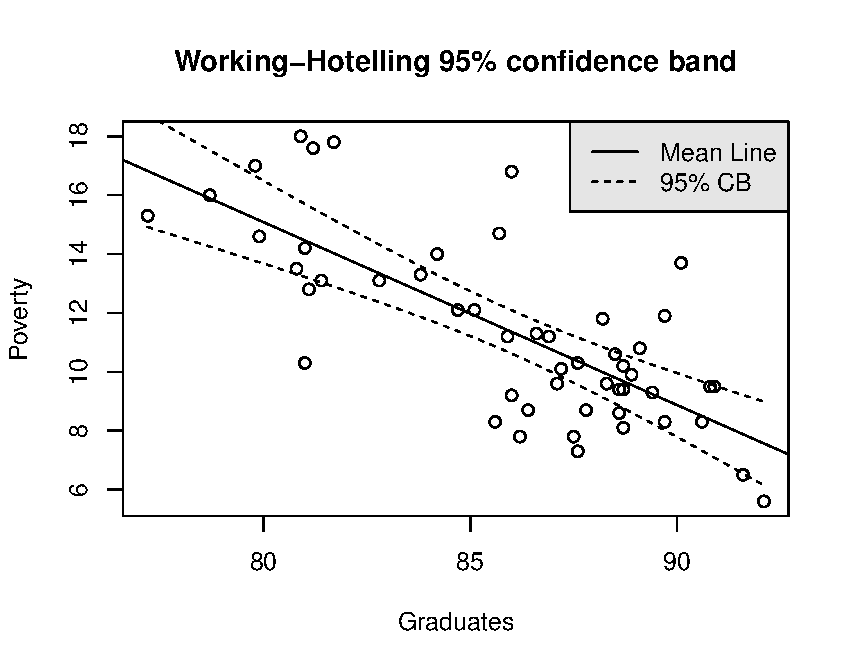
\includegraphics[width=\textwidth]{plots/conf_band.pdf}
\end{figure}
\end{column}
\end{columns}
\pause {\color{blue}\url{https://raw.githubusercontent.com/zh3nis/MATH440/main/chp02/pov_cb.R}}
\end{frame}

\section{Analysis of Variance Approach}

\begin{frame}{Decomposing $Y_i-\bar{Y}$}
Notice that
$$
\overbrace{Y_i-\bar{Y}}^{\text{Total}} = \overbrace{Y_i-\hat{Y}_i}^{\text{Error}}+\overbrace{\hat{Y}_i-\bar{Y}}^{\text{Regression}}
$$
\begin{figure}
    \centering
    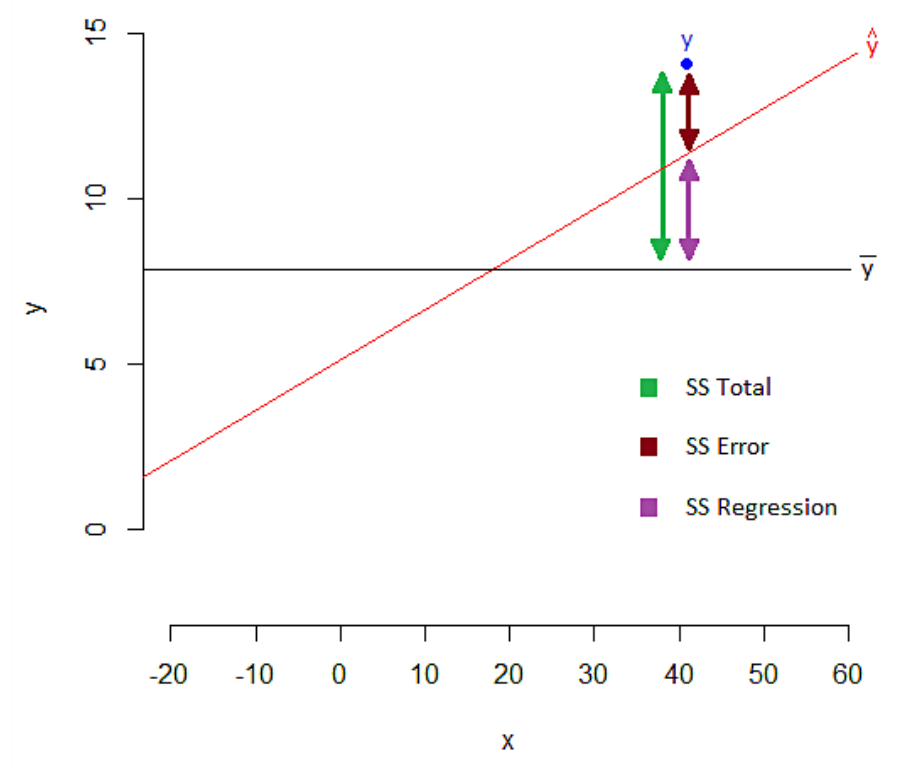
\includegraphics[width=.6\textwidth]{plots/ssto.png}
\end{figure}
\end{frame}

\begin{frame}{Partitioning SST}
\begin{equation}
\overbrace{Y_i-\bar{Y}}^{\text{Total}} = \overbrace{Y_i-\hat{Y}_i}^{\text{Error}}+\overbrace{\hat{Y}_i-\bar{Y}}^{\text{Regression}}\label{eq:tot_decomp}    
\end{equation}
\pause Squaring \eqref{eq:tot_decomp} and summing over $i$, we have
\pause$$
\underbrace{\sum(Y_i-\bar{Y})^2}_{\text{SST}}=\underbrace{\sum(Y_i-\hat{Y}_i)^2}_{\text{SSE}}+\underbrace{\sum(\hat{Y}_i-\bar{Y})^2}_{\text{SSR}}
$$
\pause because (see Chapter 1)
$$
\sum(Y_i-\hat{Y}_i)(\hat{Y}_i-\bar{Y})=\sum e_i(\hat{Y}_i-\bar{Y})=\sum e_i\hat{Y}_i-\bar{Y}\sum e_i=0
$$
\end{frame}

\begin{frame}{Degrees of Freedom of SS}
In Chapter 5 we will show that
\begin{itemize}
    \item $\frac{\text{SSE}}{\sigma^2}\sim\chi^2_{n-2}$\onslide<2->{\quad$\Rightarrow$\quad SSE has $n-2$ df}
    \item<3->$\frac{\text{SSR}}{\sigma^2}\sim\chi^2_1$ (noncentral)\onslide<4->{\quad$\Rightarrow$\quad SSR has $1$ df}
    \item<4->SSE and SSR are indep.\onslide<5->{\quad$\Rightarrow$\quad$\frac{\text{SST}}{\sigma^2}=\frac{\text{SSE}}{\sigma^2}+\frac{\text{SSR}}{\sigma^2}\sim\chi^2_{n-1}$}\onslide<6->{\pause\quad$\Rightarrow$\quad$\text{SST}$ has $n-1$ df}
\end{itemize}
\end{frame}

\begin{frame}{Expectations of SS}

\begin{prop}
$\E[\text{MSE}]=\sigma^2$.
\end{prop}
\pause{\begin{proof}
$\E[\text{MSE}]=\E\left[\frac{\text{SSE}}{n-2}\right]=\frac{\sigma^2}{n-2}\E\left[\frac{\text{SSE}}{\sigma^2}\right]=\frac{\sigma^2}{n-2}(n-2)=\sigma^2$.
\end{proof}}
\end{frame}

\begin{frame}{Expectations of SS}
\begin{prop}
$\E[\text{MSR}]=\sigma^2+\beta_1^2\sum_i{(x_i-\bar{x})^2}$.
\end{prop}
\begin{myproof}
\begin{align*}
\onslide<2->{\text{SSR}&=\sum_i(\hat{Y}_i-\bar{Y})^2=\sum_i(b_0+b_1 x_i-\bar{Y})^2\\}
\onslide<3->{&=\sum_i(\bar{Y}-b_1\bar{x}+b_1 x_i-\bar{Y})^2\pause=b_1^2\sum_i(x_i-\bar{x})^2.\\}
\onslide<4->{\E[\text{MSR}]&=\E\left[\frac{\text{SSR}}{1}\right]=\E\left[b_1^2\sum_i(x_i-\bar{x})^2\right]\\}
\onslide<5->{&=\sum_i(x_i-\bar{x})^2(\Var[b_1]+(\E[b_1])^2)\\}
\onslide<6->{&=\sigma^2+\beta_1^2\sum_i(x_i-\bar{x})^2.}
\end{align*}
\end{myproof}    
\end{frame}

\begin{frame}{Analysis of Variance (ANOVA) table}
\begin{footnotesize}
\begin{table}
\begin{tabular}{l c c c c}
\toprule
Source & SS & df & MS & $\E[\text{MS}]$\\
\midrule
Regression & $\text{SSR}=\sum(\hat{Y}_i-\bar{Y})^2$ & 1 & $\frac{\text{SSR}}{1}$ & $\sigma^2+\beta_1^2\sum(x_i-\bar{x})^2$\\
Error & $\text{SSE}=\sum(Y_i-\hat{Y})^2$ & $n-2$ & $\frac{\text{SSE}}{n-2}$ & $\sigma^2$\\
\midrule
Total & $\text{SST}=\sum(Y_i-\bar{Y})^2$ & $n-1$\\
\bottomrule
\end{tabular}
\end{table}
\end{footnotesize}
\pause\begin{remark}
$\frac{\E[\text{MSR}]}{\E[\text{MSE}]}=
\begin{cases}
1\quad&\text{if }\beta_1=0\\
>1&\text{if }\beta_1\ne0.
\end{cases}$\\~\\\pause Loosely, we expect MSR to be larger than MSE when $\beta_1\ne0$.
\end{remark}
\end{frame}

\begin{frame}{F-test for $\beta_1$}
\begin{prop}
Under $\text{H}_0:\,\beta_1=0$, we have $\frac{\text{MSR}}{\text{MSE}}\sim F_{1,n-2}$.
\end{prop}
\pause\begin{proof}
$$\frac{\text{MSR}}{\text{MSE}}=\frac{\frac{\text{SSR}}{\sigma^2}/1}{\frac{\text{SSE}}{\sigma^2}/(n-2)}=\frac{\chi^2_1/1}{\chi^2_{n-2}/(n-2)}\sim F_{1,n-2},$$
\pause because SSR and SSE are statistically independent (Ch 5).
\end{proof}
\pause\begin{remark}
The F-test and t-test for $\text{H}_0:\beta_1=0$ vs $\text{H}_1:\beta_1\ne0$ are equivalent, since\pause
$$
\frac{\text{MSR}}{\text{MSE}}=\frac{b_1^2\sum(x_i-\bar{x})^2}{\text{MSE}}=\frac{b_1^2}{\text{MSE}/\sum(x_i-\bar{x})^2}=\frac{b_1^2}{\s^2[b_1]}=\left(\frac{b_1-0}{\s[b_1]}\right)^2.
$$
\pause and both are generalized likelihood ratio tests (GLRT).
\end{remark}
\end{frame}

\begin{frame}[fragile]{ANOVA F-test in \texttt{R}}
\begin{small}
\begin{verbatim}
> poverty = read.table("path/to/poverty.txt", h = T, sep = "\t")
> my_model = lm(Poverty ~ Graduates, data=poverty)
> anova(my_model)
Analysis of Variance Table

Response: Poverty
          Df Sum Sq Mean Sq F value    Pr(>F)    
Graduates  1 267.88 267.881  61.809 3.109e-10 ***
Residuals 49 212.37   4.334               

> summary(my_model)
Coefficients:
            Estimate Std. Error t value Pr(>|t|)    
(Intercept) 64.78097    6.80260   9.523 9.94e-13 ***
Graduates   -0.62122    0.07902  -7.862 3.11e-10 ***
\end{verbatim}
\end{small}
\pause p-values of F-test and t-test for $\text{H}_0:\beta_0=0$ are same.
\end{frame}

\section{Coefficient of Determination}

\begin{frame}{Coefficient of Determination}
\begin{definition}
The \textbf{coefficient of determination} is
$$
R^2=\frac{\rm SSR}{\rm SST}=1-\frac{\rm SSE}{\rm SST},
$$
the proportion of total sample variation in $Y$ that is explained by its linear relationship with $x$.
\end{definition} 
\pause Note:
\begin{itemize}
\item $0\le R^2\le 1$.
\item $R^2=1\Rightarrow$ data perfectly linear.
\item $R^2=0\Rightarrow$ regression line horizontal ($b_1=0$).
\end{itemize}
\pause The closer $R^2$ is to one, the greater the linear relationship between $x$ and $Y$.
\end{frame}

\begin{frame}{$R^2$ for different data sets}
\begin{center}
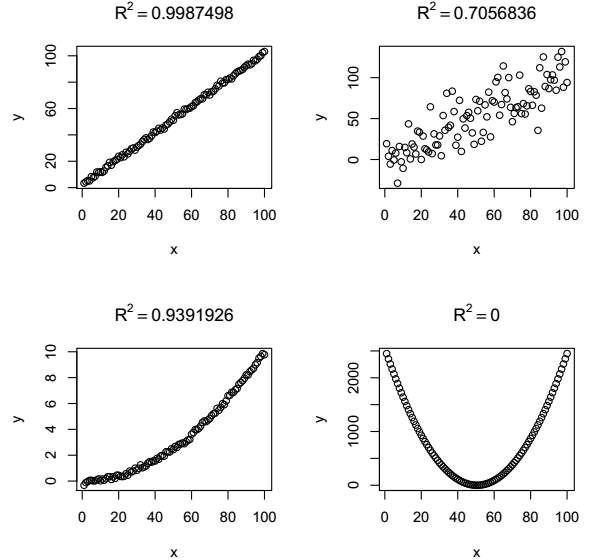
\includegraphics[scale=0.4]{plots/R-squared}
\end{center}
\end{frame}

\begin{frame}{Sample correlation $r$}
Let
$$
r=\frac{\sum_{i=1}^n(x_i-\bar{x})(Y_i-\bar{Y})}{\sqrt{\sum_{i=1}^n(x_i-\bar{x})^2\sum_{i=1}^n(Y_i-\bar{Y})^2}}
$$
be the sample correlation between $x$ and $Y$. 

\pause\begin{exe} Show that 
\begin{itemize}
    \item $R^2=r^2$,
    \item $\mathrm{sgn}(r)=\mathrm{sgn}(b_1)$.
\end{itemize}
\end{exe}

\pause\begin{remark}
\begin{itemize}
\item $r\approx 0\Rightarrow$ little linear association b/w $x$ and $Y$
\item $r\approx 1\Rightarrow$ strong positive, linear association b/w $x$ and $Y$
\item $r\approx -1\Rightarrow$ strong negative, linear association b/w $x$ and $Y$.
\end{itemize}
\end{remark}
\end{frame}

\begin{frame}[fragile]
\frametitle{Cautions about $R^2$ and $r$}
It is possible that
\begin{itemize}
\item $R^2\approx 1$, but the $\E[Y_i]$ may not lay on a line (Why?)
\item\pause $R^2\not\approx1$, but a line is best for $\E[Y_i]$ (Why?)
\item\pause $R^2\approx 0$, but $x$ and $Y$ are highly related (Why?)
\end{itemize}

\vspace{20pt}
\pause Poverty vs HS Graduation data:
\begin{small}
\begin{verbatim}
> summary(my_model)
...
Residual standard error: 2.082 on 49 degrees of freedom
Multiple R-squared:  0.5578, Adjusted R-squared:  0.5488 
F-statistic: 61.81 on 1 and 49 DF,  p-value: 3.109e-10
\end{verbatim}
\end{small}
\end{frame}


\begin{frame}{Cautions about regression}
\begin{itemize}
\item Concluding that $x$ and $Y$ are linearly related (that $\beta_1\ne0$) does not imply a causal relationship between $x$ and $Y$. \onslide<2->{(Correlation does not imply causation!)}
\item<3-> Beware of extrapolation: predicting $Y$ for $x$ far outside the range of $x$ in the data. The relationship may not hold outside of the observed $x$-values.
\begin{itemize}
\item<4-> Sometimes the intercept might be an extrapolation.
\end{itemize}
\end{itemize}
\onslide<5->{\begin{center}
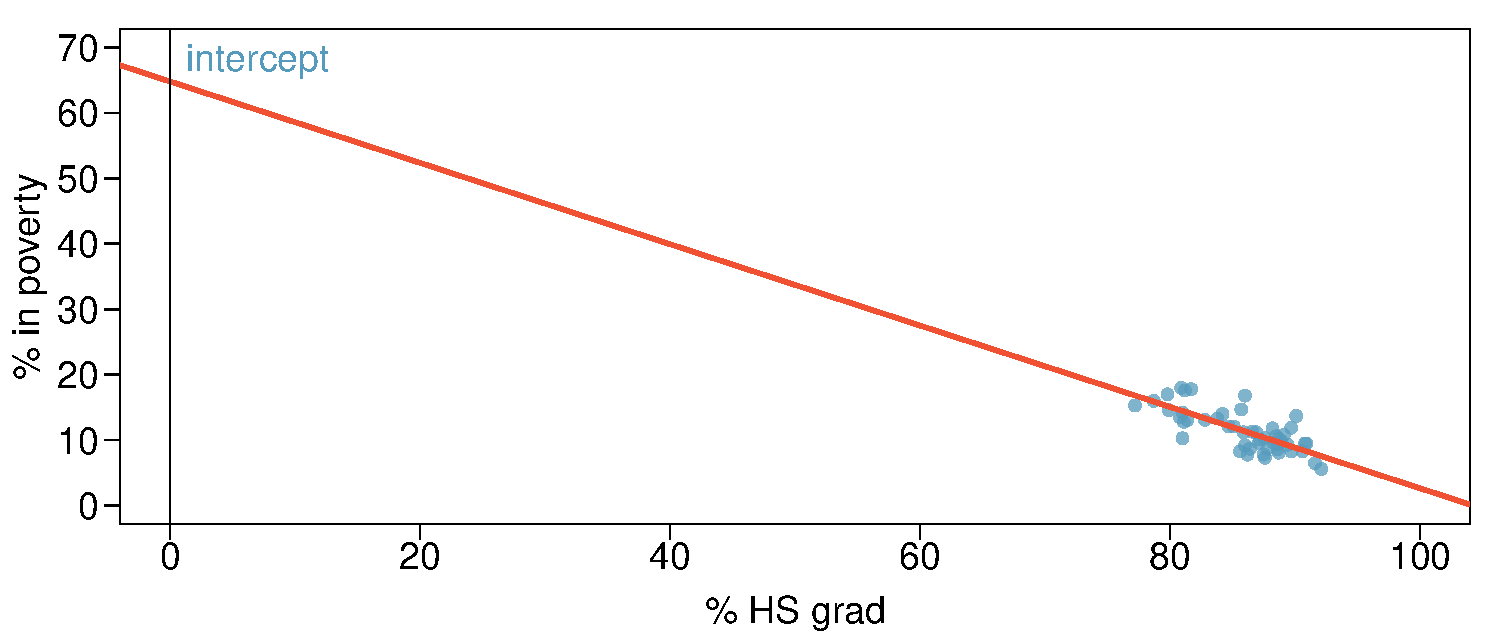
\includegraphics[width=.8\textwidth]{plots/poverty_hsgrad_line_wide}
\end{center}}
\end{frame}

%%%%%%%%%%%%%%%%%%%%%%%%%%%%%%%%%%

\begin{frame}
\frametitle{Examples of extrapolation}

\begin{center}
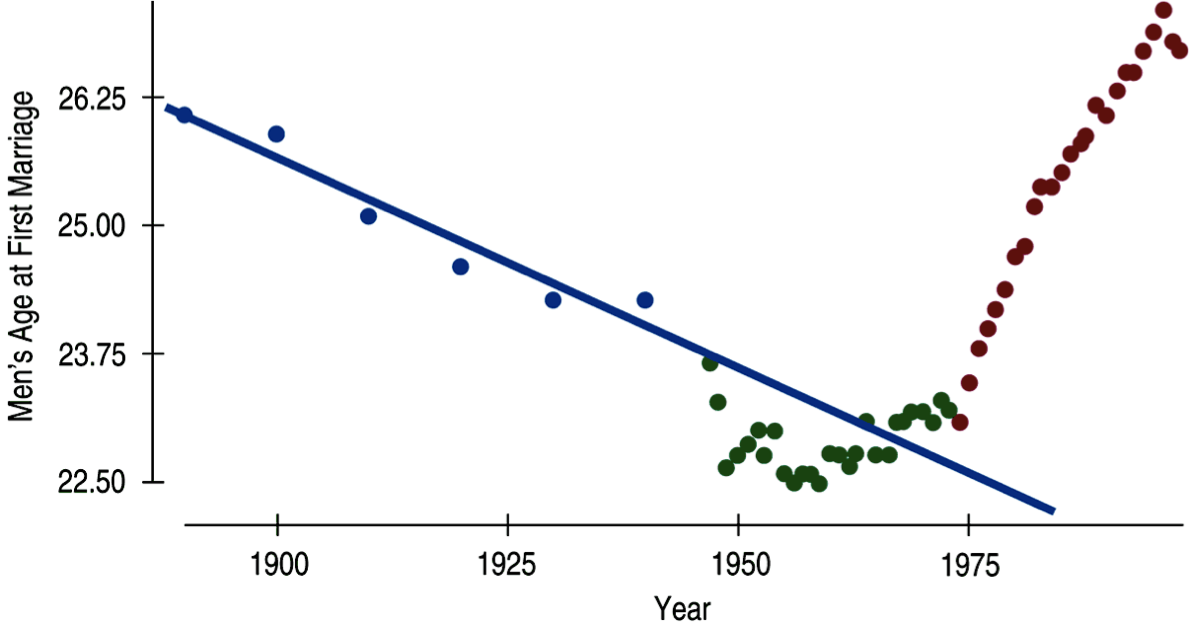
\includegraphics[width=\textwidth]{plots/extrapolation}
\end{center}

\end{frame}

%%%%%%%%%%%%%%%%%%%%%%%%%%%%%%%%%%

\begin{frame}
\frametitle{Examples of extrapolation}

\begin{center}
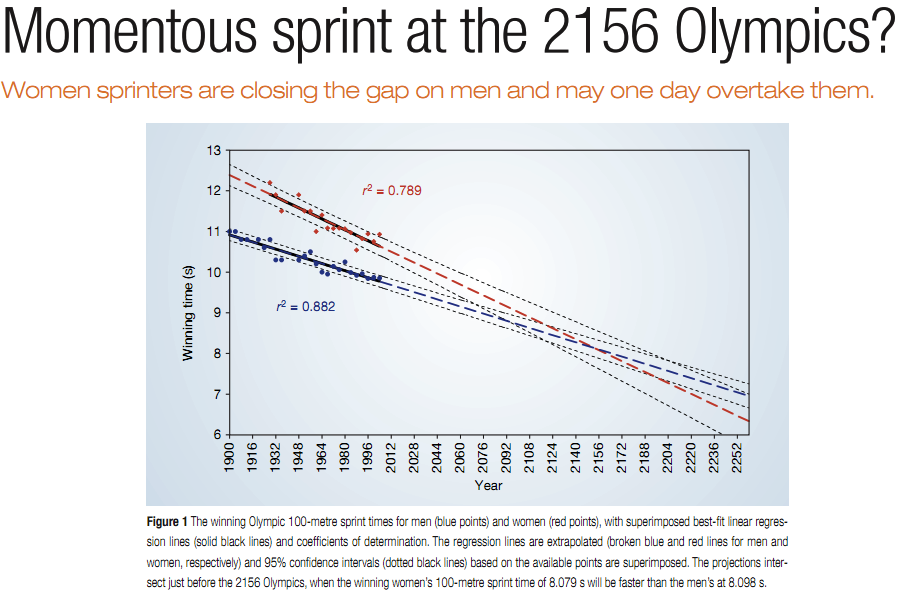
\includegraphics[width=\textwidth]{plots/womenOutsprint}
\end{center}

\end{frame}

\end{document}